\documentclass[a4paper, 12pt]{article}
\usepackage[total={17cm,25cm}, top=2.5cm, left=2.5cm, right=2.5cm,  includefoot]{geometry}
\usepackage[utf8]{inputenc}
\usepackage{array}
\usepackage{multirow}
\usepackage{hhline}
\usepackage{gensymb}
\usepackage{graphicx}
\graphicspath{ {} }
\usepackage[czech]{babel}
\usepackage{enumitem}
\usepackage{pdfpages}
\usepackage{amsmath}
\usepackage{verbatim}
\usepackage{listings}
\usepackage{hyperref}
\usepackage{amssymb}


\pagestyle{empty} % vypne číslování stránek




\usepackage[OT2,OT1]{fontenc}
\newcommand\cyr
{
\renewcommand\rmdefault{wncyr}
\renewcommand\sfdefault{wncyss}
\renewcommand\encodingdefault{OT2}
\normalfont
\selectfont
}
\DeclareTextFontCommand{\textcyr}{\cyr}
\def\cprime{\char"7E }
\def\cdprime{\char"7F }
\def\eoborotnoye{\char’013}
\def\Eoborotnoye{\char’003}


\begin{document}



\begin{titlepage}
\begin{center}
\noindent
\Large \textbf{České vysoké učení technické v Praze }\\ Fakulta stavební
\vspace{5cm}

\huge

%vložení loga cvut
\begin{figure}[h!]
	\centering
	
\includegraphics[width=7cm]{logo.png}
\end{figure}

\vspace{0.5cm}

Algoritmy v digitální kartografii \\

\vspace{3cm}

\Huge  
Geometrické vyhledávání bodu\\

\vspace{2cm}

\Large
Bc. Robin Pflug \\
Bc. Tomáš Klemsa \\

\end{center}

\end{titlepage}




\pagestyle{plain}     % zapne obyčejné číslování
\setcounter{page}{1}  % nastaví čítač stránek znovu od jedné

\tableofcontents
\newpage

\section{Zadání úlohy}

\textbf{Vstup:} \textit{Souvislá polygonová mapa n polygonů ${P1, ..., Pn}$, analyzovaný bod q.}\\
\textbf{Výstup:} 	$P_i , q \epsilon P_i$\\

Nad polygonovou mapou implementujete následující algoritmy pro geometrické vyhledávání:
\begin{itemize}
  \item Ray Crossing Algorithm (varianta s posunem těžiště polygonu).
  \item Winding Number Algorithm.
\end{itemize}

Nalezený polygon obsahující zadaný bod q graficky zvýrazněte vhodným způsobem (např. vyplněním, šrafováním, blikáním). Grafické rozhraní vytvořte s využitím frameworku QT.\\
\\
Pro generování nekonvexních polygonů můžete navrhnout vlastní algoritmus či použít existující
geogracká data (např. mapa evropských států).\\
\\
Polygony budou načítány z textového souboru ve Vámi zvoleném formátu. Pro datovou reprezentaci jednotlivých polygonů použijte špagetový model.

\begin{figure}[h!]
	\centering
	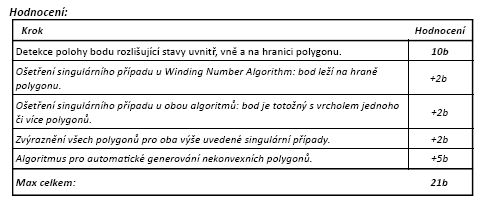
\includegraphics[width=16cm]{hodnoceni.jpg}
	\caption{Bodové hodnocení úlohy [zdroj: 1]}
\end{figure}

\clearpage

\section{Obecná formulace a řešení problému}
Ve 2D souřadnicích je dána množina n vrcholů, m polygonů a bod q.
Cílem řešení problému je určit takový polygon (mnohoúhelník), který bod q obsahuje. V případě
řešení bonusových úloh je cílem nalézt takové polygony, jejichž hrana či vrchol obsahují bod q.
Řešení je určeno pro nekonvexní polygony. Testu polohy bodu q vůči polygonu je za realizován pomoci
lokální procedury (tj. opakované určení polohy bodu q vzhledem k polygonu).\\
\\
Základním zadáním úlohy bylo určit vzájemnou polohu bodu a polygonů. Problém byl řešen dvěma
způsoby: algoritmem využívajícího Winding Number a algoritmem nazývaným Ray Crossing. Řešení
problematiky je implementováno s využitím Widgedts aplikace napsané v jazyce C++. Aplikace byla
tvořena na platformě Qt Creator v operačním systému Windows.\\
\\
Prvním krokem před samotnou tvorbou aplikace byla tvorba kostry programu. Bylo nutné oddělit
funkce provádějící přípravu dat a samotný výpočet algoritmů od funkcí zajišťujících chod grafického
rozhraní, vstupu apod.\\
\\
Pro aplikaci bylo nejprve navrženo základní grafické okno, které bylo postupně doplňováno o
potřebné interaktivní prvky (především push buttony apod.). Pro zpracování grafické funkcionality vstupu a výstupu dat byla vytvořena třída Draw. Pro funkce zpracovávající oba algoritmy byla vytvořena třída Algorithms. Načítání externích dat (polygonů) je prováděno ve třídě filereader.\\
\\
Konkrétní řešení a vzorce použité při řešení problematiky jsou obsahem následujících kapitol.

\section{Aplikované algoritmy}
Algoritmy využívané pro geometrické vyhledávání bodu.

\subsection{Winding Algorithm}
Algoritmus vychází z výpočtu úhlů mezi jednotlivými
průvodiči z analyzovaného bodu q do jednotlivých vrcholů $p_i$ příslušného polygonu P. Postupným přičítáním a odčítáním úhlů (podle směru z předchozího pi na následující vrchol $p_{i+1}$ polygonu P) mezi průvodiči je získávána informace, kde se bod q vůči polygonu P nachází. Zda se úhel mezi průvodiči do výsledné sumy úhlů přičte či
odečte udává polorovina, ve které se úhel vůči spojnici z bodu q do vrcholu polygonu $p_i$ nachází.
Úhly nacházející se v pravé, takto definované polorovině, jsou orientovány kladně a proto se
přičítají. Úhly v levé polorovině se odčítají. Na základě výsledné sumy všech úhlů pro daný polygon
P mohu určit polohu bodu q. Je-li suma úhlů násobkem $2\pi$ znamená to, že bod q se nachází uvnitř
polygonu P, je-li úhel menší (důsledek odčítání záporně orientovaných úhlů), bod q leží vně
polygonu P.\\
\\
Winding number je udáváno jako násobek $2\pi$(v radiánové míře). Výsledná hodnota winding
number závisí na orientaci směru pohybu (CW x CCW).

\begin{figure}[h!]
	\centering
	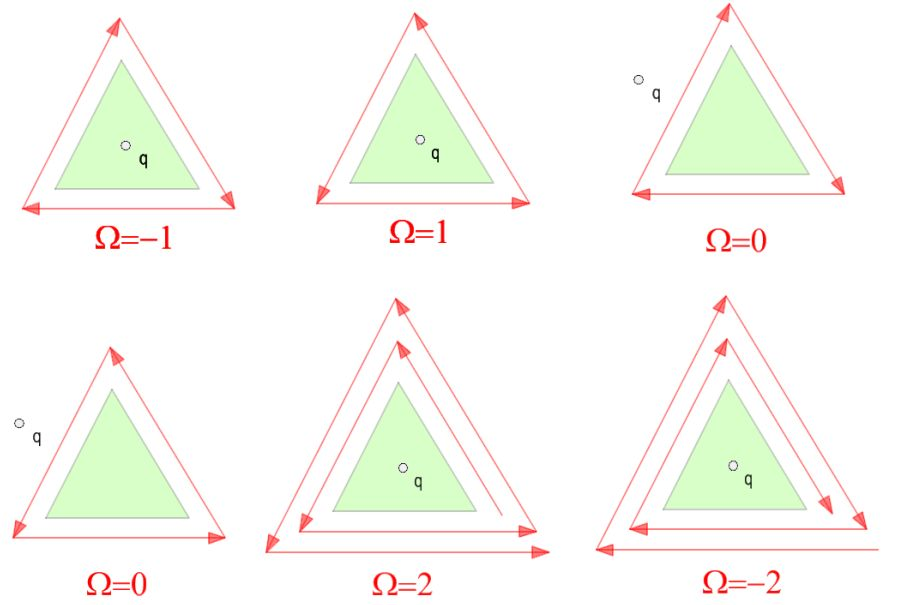
\includegraphics[width=12cm]{winding.jpg}
	\caption{Princip výpočtu winding number [zdroj: 1]}
\end{figure}

\subsubsection{Algoritmus winding number}
\begin{enumerate}
\item Inicializace $\Omega = 0$, tolerance $\epsilon$
\item Opakuj pro $ \forall $ trojici $ (p_i, q, p_{i+1}): $
\subitem Urči polohu q vzhledem k $e_i = (p_i, p_{i+1}).$
\subitem Urči úhel $ \omega_i = \angle p_i, q, p_{i+1}.$
\subitem If $ q \epsilon \overline{\sigma}_l, $ pak $ \Omega = \Omega + \omega_i. $
\subitem else $ \Omega = \Omega - \omega_i.$
\item if $ \Vert \omega \vert - 2\pi \vert < \epsilon, $ pak $ q \epsilon P. $
\item else $ q \notin p.$
\end{enumerate}[zdroj: 1]

\subsection{Ray crossing}
Základem Ray crossing algoritmu je přímka r procházející analyzovaným bodem q. Poloha bodu q
vůči polygonu P je určována na základě počtu průsečíků přímky k a hran polygonu $p_i$. Obecně platí pro bod q vně polygonu P, že počet průsečíků k je sudý, lichý počet k platí pro bod q uvnitř polygonu P. Problém singularit pro takto daný model algoritmu je řešen převedením na upravený model. V upraveném modelu algoritmu je pro určení výsledku uvažována pouze jedna polorovina vzhledem k paprsku r procházejícím bodem q. Další modifikace redukuje souřadnice vrcholů pi polygonu P k analyzovanému bodu q. Pro model s takto vytvořenou lokální souřadnicovou
soustavou jsou hledány pouze průsečíky M ležící v pravé polorovině od osy x, která po redukci prochází bodem q. Výsledná varianta algoritmu tedy uvažuje pouze průsečíky M ležící v jednou
kvadrantu (v popisovaném případě se jedná o první kvadrant) lokální souřadnicové soustavy vzhledem k bodu q. Takto upravený algoritmus

\begin{figure}[h!]
	\centering
	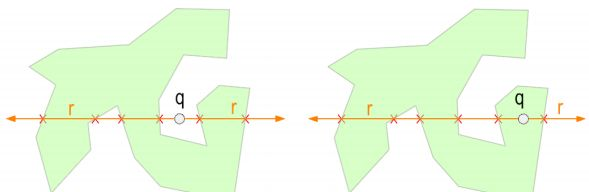
\includegraphics[width=12cm]{raz.jpg}
	\caption{Princip Ray crossing algoritmu [zdroj: 1]}
\end{figure}

\subsubsection{Algoritmus Ray crossing s redukcí}
\begin{enumerate}
\item Inicializuj $k = 0$
\item Opakuj pro $ \forall $ body $ p_i \epsilon P: $
\subitem  $ x'_i = x_i - x_q $
\subitem  $ y'_i = y_i - y_q $
\subitem  if $ (y'_i > 0)$ \&\& $(y'_{i-1} <= 0)||(y'_i <= 0)$\&\&$(y'_{i-1} > 0)$
\subitem $ x'_m = (x'_i y'_{i-1} - x'_{i-1} y'_i)/(y'_i - y'_{i-1}) $
\subitem if $ (x'_m > 0) pak k = k+1 $
\item if $(k \mod 2) \neq 0$ pak $q \epsilon P $
\item else $ q \notin p.$
\end{enumerate} [zdroj: 1]

\section{Vstup dat do aplikace}
\textbf{\textit{Vstup dat lze provádět:}}\\
Grafickým vstupem, kdy jsou snímány souřadnice bodů kurzorem myši v grafickém rozhraní aplikace.\\
\\
Kombinovaným vstupem, kde jsou souřadnice polygonů načítány z textového souboru v předepsaném formátu a souřadnice analyzovaného bodu jsou snímány kurzorem myši v grafickém rozhraní aplikace.\\
\\
Třetím způsobem vstupu dat do aplikace, konkrétně polygonu, je automatická generace. Tento způsob vstupu je obsahem bonusových úloh. Tlačítkem \textit{Generate Random Polygon} lze vygenerovat v grafickém okně polygon o náhodném počtu vrcholů od 4 do 20. Vstup tímto způsobem nefunguje v aplikace správně a pro především větší počet vrcholů, generuje topologicky nekorektní polygony.

\subsection{Grafický vstup}
Grafický vstup vrcholů polygonu je aktivován tlačítkem Polygon v sekci Draw Action. Pro ukončení snímání aktuálního polygonu je třeba aktivovat tlačítko None. Poté lze opět po aktivaci tlačítka Polygon snímat a vykreslovat nový polygon nebo aktivací tlačítka Analyze point snímat souřadnice analyzovaného bodu.

\subsection{Kombinovaný vstup}
Pro načtení polygonů z textového souboru je určena sekce Import s tlačítkem Import polygons. Po aktivaci tlačítka lze v dialogovém okně vybrat příslušný soubor a nahrát polygony hromadně do aplikace.

\subsection{Formát souboru pro import dat}
Každý polygon začíná číslem vrcholu od čísla 1 po odsazení tabulátorem následuje souřadnice x, po dalším odsazením souřadnice y. Jednotlivé vrcholy jsou odřádkovány. Nový polygon začíná opět číslem vrcholu 1.

\begin{figure}[h!]
	\centering
	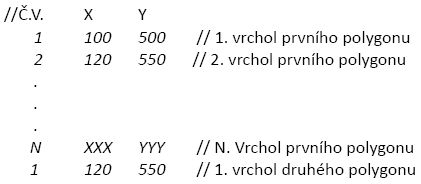
\includegraphics[width=8cm]{vstup.jpg}
	\caption{Příklad formátu vstupních souřadnic}
\end{figure}

\section{Výstup aplikace}
Výstupní data jsou prezentována grafickou cestou. Po zadání souřadnic polygonů a analyzovaného bodu jsou vstupní data vykreslena v grafickém okně. Po aktivaci tlačítka Polygon point pozition analyze je graficky zvýrazněn červenou barvou polygon, ve kterém se bod nachází. Nachází-li se bod na hraně či vrcholu polygonu, je polygon zvýrazněn zelenou barvou.

\begin{figure}[h!]
	\centering
	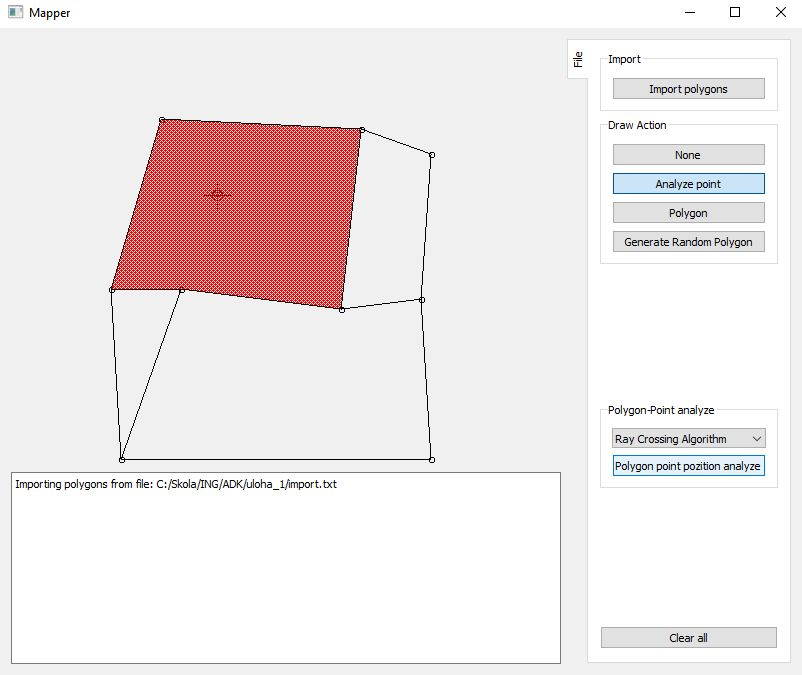
\includegraphics[width=12cm]{vystup1.jpg}
	\caption{Výstup aplikace pro analýzu metodou Ray Crossing}
\end{figure}

\begin{figure}[h!]
	\centering
	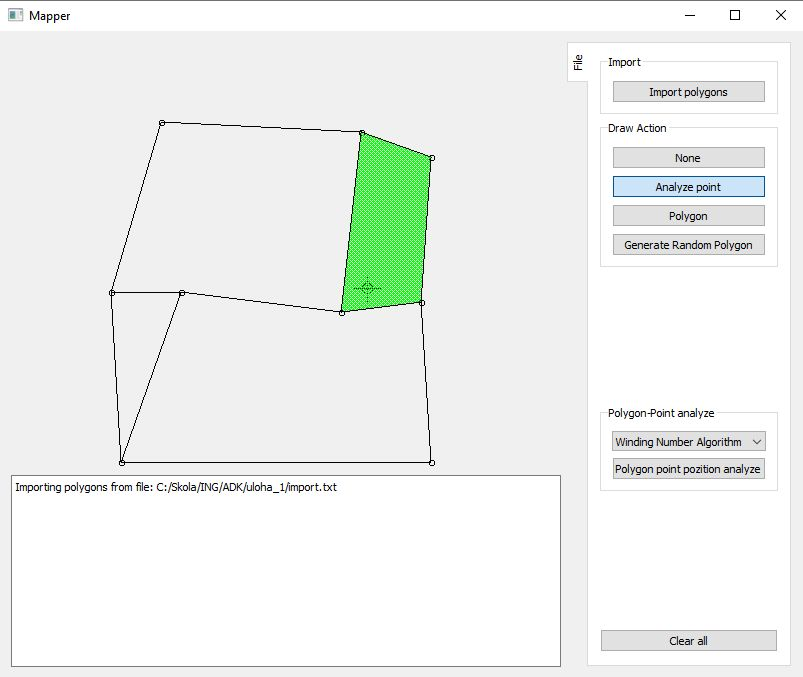
\includegraphics[width=12cm]{vystup2.jpg}
	\caption{Výstup aplikace pro analýzu metodou Winding number}
\end{figure}

\begin{figure}[h!]
	\centering
	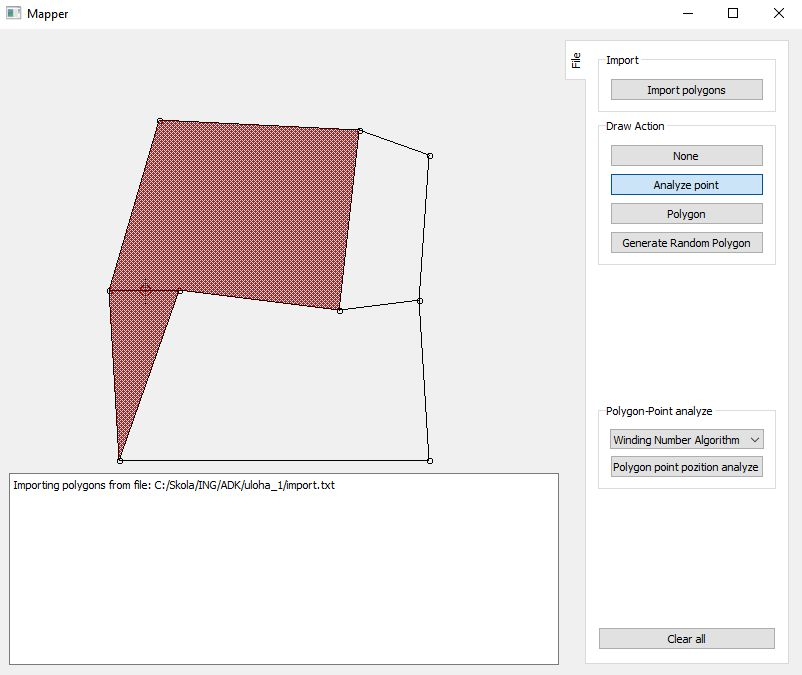
\includegraphics[width=12cm]{vystup3.jpg}
	\caption{Výstup aplikace pro analýzu, kdy se bod nachází na hraně dvou polygonů}
\end{figure}

\begin{figure}[h!]
	\centering
	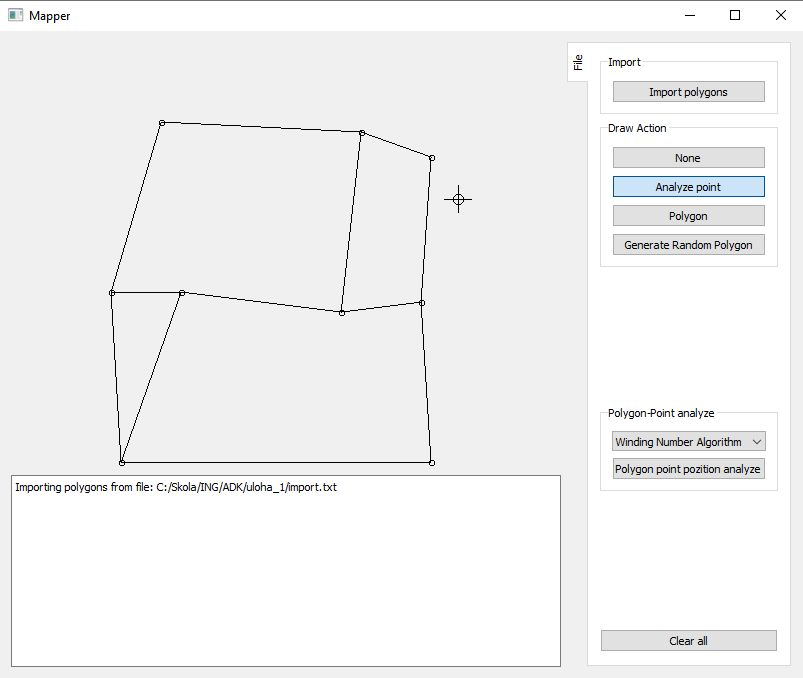
\includegraphics[width=12cm]{vystup4.jpg}
	\caption{Výstup aplikace pro analýzu bodu, který nenáleží žádnému polygonu}
\end{figure}

\clearpage
\section{Dokumentace}
\subsection{Třídy}
\subsubsection{Algorithms}
Třída obsahující metody potřebné pro výpočet polohy bodu vzhledem k polygonu.
\\

\textbf{int getPointLinePosition(QPointF q,QPointF p1,QPointF p2)}\\
Návratová hodnota: \textit{integer};\\
Určení polohy bodu vůči přímce. Návratová hodnota
1 pro bod v levé polorovině, 0 pro bod v pravé
polorovině, -1 pro bod na přímce.\\
\\

\textbf{double getAngle2Vectors(QPointF p1,QPointF p2,QPointF p3,QPointF p4)}\\
Návratová hodnota: \textit{double};\\
Metoda vrací úhel mezi dvěma vektory.\\
\\

\textbf{int positionPointPolygonWinding(QPointF q, QPolygonF pol)}\\
Návratová hodnota: \textit{integer};\\
Obsahuje Winding number algoritmus pro
výpočet polohy bodu vůči polygonu.
Návratová hodnota 1 pro body v polygonu, 0
pro bod mimo polygon a -1 pro bod na hraně
polygonu.\\
\\

\textbf{int positionPointPolygonRayCrossing(QPointF q, QPolygonF pol)}\\
Návratová hodnota: \textit{Integer};\\
Obsahuje Ray crossing algoritmus pro
výpočet polohy bodu vůči polygonu.
Návratová hodnota 1 pro body v polygonu, 0
pro bod mimo polygon a -1 pro bod na hraně
polygonu.\\
\\

\textbf{QPolygonF createRandomPolygon()}\\
Návratová hodnota: \textit{QPolygonF};\\
Metoda generující náhodný polygon o 4 až 20
vrcholech.

\subsubsection{Draw}
Třída s metodami zajišťující snímání a ukládání dat grafického vstupu. Metody také zajišťují grafické vykreslení dat. Třída také umožňuje přepínání metod grafického vstupu.

\subsubsection{FileReader}
Třída obsahující funkce zajišťující import polygonů v podobě textového souboru.

\subsubsection{Widget}
Třída vytvářející grafické rozhraní aplikace.

\section{Řešení bonusových úloh}
Z bonusových úloh bylo řešeno zadání: \textit{Algoritmus pro automatické generování nekonvexních polygonů} a \textit{Ošetření singulárního případu u Winding Number Algorithm: bod leží na hraně polygonu.}.

\subsubsection{Ošetření singulárního případu u Winding Number Algorithm: bod leží na hraně polygonu}
Tento singulární případ byl ošetřen při určování pozice bodu vůči přímce (funkce: \textit{getPointLinePosition}). Funkce vyhodnotí jako kolineární bod \textit{q}  takový, který má součet vzdáleností počátečního bodu úsečky do \textit{q} (p1,q) a \textit{q} do koncového bodu úsečky (q,p2) krajně blízký k samotné délce úsečky (p1,p2).

\subsubsection{Algoritmus pro automatické generování nekonvexních polygonů}
Automatické generování nekonvexních, topologicky korektních polygonů se nepodařilo správně naimplementovat (viz \textit{Náměty pro vylepšení}). 

\section{Závěr}
Pro předpřipravená data aplikace funguje bez problému, problematické situace algoritmu podle
zadání byly ošetřeny. Aplikace umožňuje několik metod vstupů dat a pro povinnou část zadání vyhodnocuje analýzu správně.

\section{Náměty pro vylepšení} 
Algoritmus pro automatické generování polygonů se nepodařilo správně naimplementovat. Algoritmus nevytváří vždy topologicky korektní polygony.\\
\\
Aplikacke by byla o mnoho všestrannější, pokud by při importu neupravených polygonů z textového souboru, automaticky redukovala souřadnice vrcholů tak, aby je bylo možné zobrazit v grafickém okně. Tento problém aplikace neřeší a proto je nutné před importem souřadnice upravit jiným způsobem.

\section{Reference}

\begin{enumerate}

\item  BAYER, Tomáš. Metody konstrukce konvexní obálky [online][cit. 5.11.2019]. \\
Dostupné z: https://web.natur.cuni.cz/~bayertom/images/courses/Adk/adk4.pdf  \\

\end{enumerate}
\end{document}



 